\documentclass[landscape]{article}
\pagenumbering{gobble}

\usepackage[a4paper]{geometry}
\usepackage[utf8]{inputenc}
\usepackage{tikz}
\usepackage[compat=1.1.0]{tikz-feynman}
\usepackage{graphicx}

\begin{document}
\centering
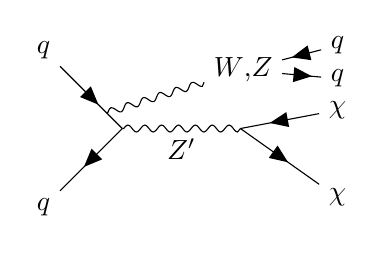
\begin{tikzpicture}
  \begin{feynman}
    % initial state particles
    \vertex (i1) {\(q\)};
    \vertex [below=2cm of i1] (i2) {\(q\)};

    % vertices
    \vertex [below right=1cm and 1cm of i1] (a);
    \vertex [right=1.5cm of a] (b);

    % final state particles
    \vertex [above right=.0cm and 1cm of b] (f1) {\(\chi\)};
    \vertex [below right=.64cm and 1cm of b] (f2) {\(\chi\)};
    \vertex [above left=0.51cm and 1.2cm of f1] (r) {$W$,$Z$};
    \vertex [above right=0.31cm and 1.2cm of r] (f3) {$q$};
    \vertex [below right=0.11cm and 1.2cm of r] (f4) {$q$};


    \diagram* {
      (i1) -- [fermion] (a)
        -- [fermion] (i2),

      (a) -- [boson, edge label'=\(Z'\)] (b),

      (f1) -- [fermion] (b)
        -- [fermion] (f2),

       (f3) -- [fermion] (r)
        -- [fermion] (f4),
    };
      \draw [boson] ($(i1)!0.8!(a)$) -- (r);
  \end{feynman}
\end{tikzpicture}%
\end{document}
